\documentclass[border=10pt]{standalone}
\usepackage{pgfplots}
\usepgfplotslibrary{colormaps}
\pgfplotsset{compat=newest}

\begin{document}
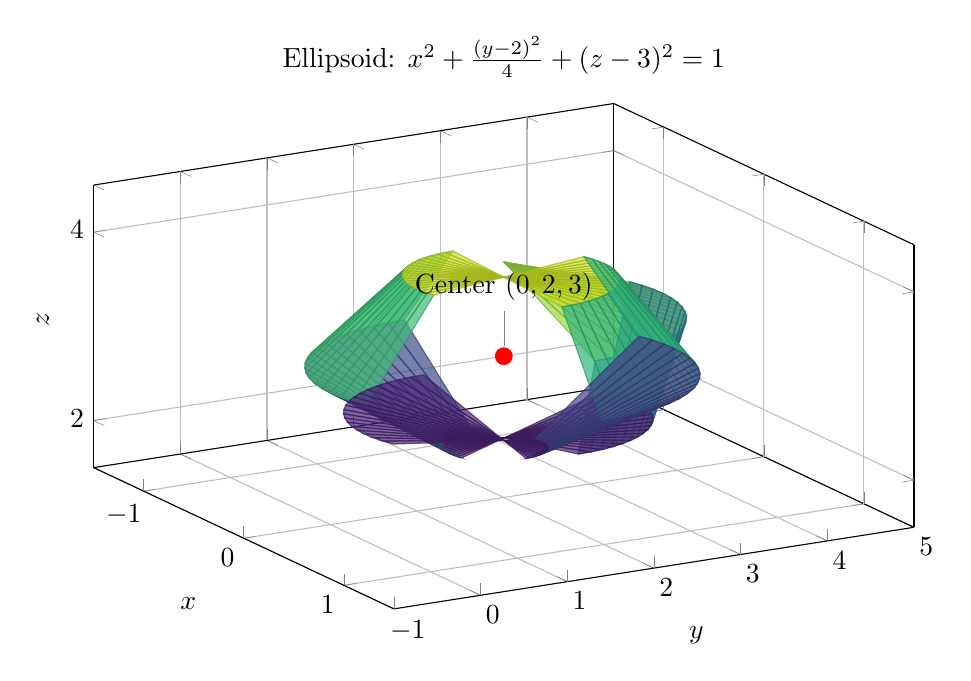
\begin{tikzpicture}
\begin{axis}[
    view={60}{30},
    xlabel={$x$},
    ylabel={$y$},
    zlabel={$z$},
    title={Ellipsoid: $x^2 + \frac{(y-2)^2}{4} + (z-3)^2 = 1$},
    colormap/viridis,
    grid=major,
    xmin=-1.5, xmax=1.5,
    ymin=-1, ymax=5,
    zmin=1.5, zmax=4.5,
    width=12cm,
    height=8cm
]
\addplot3[
    surf,
    domain=0:360,
    y domain=0:180,
    samples=20,
    samples y=10,
    opacity=0.7
] (
    {sin(deg(y))*cos(deg(x))},
    {2 + 2*sin(deg(y))*sin(deg(x))},
    {3 + cos(deg(y))}
);

\addplot3[only marks, mark=*, mark size=3, red] coordinates {(0, 2, 3)};
\node[pin={above:Center $(0,2,3)$}] at (axis cs:0,2,3) {};

\end{axis}
\end{tikzpicture}
\end{document}
